%$Header: /cvsroot/esrg/sfesrg/esrgpcpj/hyreach/doc/hyreachm/s_iop0/s_iop0.tex,v 1.11 2002/01/29 17:04:00 dtashley Exp $
%
\section{Internal Operation Of The Software}
\label{siop0}

This section describes aspects of the internal operation of the software
which may be useful when trying to understand the source code, trying to
understand why \swname{} is not behaving as expected, or when creating
separate software with similar functionality.


%%%%%%%%%%%%%%%%%%%%%%%%%%%%%%%%%%%%%%%%%%%%%%%%%%%%%%%%%%%%%%%%%%%%%%%%%%%%%%%
%%%%%%%%%%%%%%%%%%%%%%%%%%%%%%%%%%%%%%%%%%%%%%%%%%%%%%%%%%%%%%%%%%%%%%%%%%%%%%%
%%%%%%%%%%%%%%%%%%%%%%%%%%%%%%%%%%%%%%%%%%%%%%%%%%%%%%%%%%%%%%%%%%%%%%%%%%%%%%%
\subsection[Implementation Of Convex Regions Of $\mathbb{R}^N$]
           {Implementation Of Convex Regions Of \mbox{\boldmath $\mathbb{R}^N$}}
%Subsection Tag: IRN0
\label{siop0:sirn0}

The fundamental data structure used for verification is a subset of
$\mathbb{R}^N$ bounded by a number of inequalities of the form

\begin{equation}
\label{eq:siop0:sirn0:01}
x_i - x_j \;\; \{<|\leq\} \;\; d_{ij},
\end{equation}

\noindent{}where the vertical bar (``$|$'') is used to denote that either
``$<$'' or ``$\leq$'' may be chosen as the relational operator.
We call an inequality in the form of (\ref{eq:siop0:sirn0:01})
an \index{atomic constraint}\emph{atomic constraint}.
Our implementation is a form of difference bound matrix (or DBM)
such as is discussed in 
\cite[Section 17.6, p. 287]{bib:b:modelchecking:clark1999} and also
in numerous other places throughout timed automata literature.

We call the region of $\mathbb{R}^N$ described by a set of
inequalities in the form of (\ref{eq:siop0:sirn0:01}) conjuncted
together
a \index{convex zone}\emph{convex zone}.  The term
\emph{convex} is natural to apply since it is provable that
such a region of $\mathbb{R}^N$ is convex.  The term
\index{zone}\emph{zone} comes from timed automata literature.
In this section, just a few important properties 
and one special case of convex zones
are discussed.

The fundamental data structure employed by \swname{} is a list of
constraints in the form of (\ref{eq:siop0:sirn0:01}), conjuncted
(and'd) together.  

The C-language definition of each atomic constraint is described by
the code in Figure \ref{fig:siop0:sirn0:01}.  Note that the 
constraint has a bitfield to signal that $\leq$ rather than
$<$ applies, and a flag to signal that the constraint is used
(during some operations, the constraints may become non-contiguous---the
flag is used to mark some constraints for removal before the array of
constraints is compacted).  Note also that $x_0$ is taken to be 
0 to allow manipulation of constraints in a uniform framework, 
as is done in much of the literature.

\begin{figure}
\begin{small}
\begin{verbatim}
/* Defines a single constraint, i.e. x[a]-x[b] <|<= K as known
** to this module.  x[0] is always the value of zero.  Any given
** convex region or zone is a conjunction of such inequalities.
*/
typedef struct
   {
   unsigned valid   :   1;
      /* TRUE if record is valid, i.e. used.
      */
   unsigned eq      :   1;
      /* TRUE if the inequality is <= rather than
      ** <.
      */
   int v1; 
   int v2;
      /* Subscripts of variables in v1 - v2 <|<= k.
      */
   int k;
      /* The constant involved.
      */
   } CVXZONE_constraint, *CVXZONE_constraint_ptr;
\end{verbatim}
\end{small}
\caption{C-Language Data Structure For Constraint}
\label{fig:siop0:sirn0:01}
\end{figure}

The C-language definition of a convex zone is given by the 
code in Figure \ref{fig:siop0:sirn0:02}.  Since a convex zone
is taken to be the conjunction of all of the existing constraints,
a convex zone with no constraints is interpreted as $\mathbb{R}^N$.
This also gives a convenient way to specify infinite spaces, as 
some constraints are simply omitted.
However, except for the awkward idea of intentionally
specifying contradictory
constraints, no way exists (using only constraints) to specify
the empty set, and so a flag is included in the structure to 
signal the empty set.  Thus the canonical form of $\mathbb{R}^N$
is a convex zone with no constraints, and the canonical form
of the empty set is a convex zone with no constraints, but with the
\texttt{is\_empty} flag set.

\begin{figure}
\begin{small}
\begin{verbatim}
typedef struct
   {
   unsigned is_canonical : 1;
      /* TRUE if the data structure is in canonical form.  This
      ** flag is maintained so that repeated needs to put in
      ** canonical form will not take any CPU time.  Essentially
      ** any operation that modifies this data structure will
      ** violate the canonical form and cause this flag to be
      ** set to 0.
      */
   unsigned is_empty     : 1;
      /* By default, a space with no constraints is taken to be
      ** full, i.e. to contain all of R-space.  This flag negates
      ** that, i.e. signals the empty set.  The canonical form
      ** of all-space is no constraints and this flag FALSE.  The
      ** canonical form of no-space is no constraints and this
      ** flag TRUE.
      */
   unsigned n_allocd;
      /* The number of slots allocated for constraints in this
      ** data structure.  This value grows, but never shrinks.
      ** This is the number allocated, but not necessarily the
      ** number used.  This value grows in steps of 
      ** CVXZONE_ZONE_CONST_ALLOC_INC.  If this value is zero,
      ** the pointer below must be NULL.
      */
   unsigned n_used;
      /* The number of slots which are used.  This means that the
      ** used slots range from 0 through this value - 1.
      ** This only flags the constraints which must be inspected
      ** and potentially apply, but not necessarily every constraint
      ** in this range applies.  In addition to the constraint being
      ** subscripted in 0..n-1, the constraint must also have its
      ** valid bit set.  The set of active constraints is thus
      ** those in the range of 0..n-1 with their valid bits set.
      */
   CVXZONE_constraint_ptr constraints;
      /* Pointer to the allocated block of constraints.  The number
      ** allocated is realloc'd up by CVXZONE_ZONE_CONST_ALLOC_INC
      ** slots each time one runs out of memory.
      */
   } CVXZONE_zone, *CVXZONE_zone_ptr;
\end{verbatim}
\end{small}
\caption{C-Language Data Structure For Convex Zone}
\label{fig:siop0:sirn0:02}
\end{figure}

Note also in Figure \ref{fig:siop0:sirn0:02}
that that maintaining an array of constraints involves two sizes:
\texttt{n\_used} and \texttt{n\_allocd}.  By default,
the memory allocated for the array of constraints never shrinks.


%%%%%%%%%%%%%%%%%%%%%%%%%%%%%%%%%%%%%%%%%%%%%%%%%%%%%%%%%%%%%%%%%%%%%%%%%%%%%%%
%%%%%%%%%%%%%%%%%%%%%%%%%%%%%%%%%%%%%%%%%%%%%%%%%%%%%%%%%%%%%%%%%%%%%%%%%%%%%%%
%%%%%%%%%%%%%%%%%%%%%%%%%%%%%%%%%%%%%%%%%%%%%%%%%%%%%%%%%%%%%%%%%%%%%%%%%%%%%%%
\subsubsection{Implication Among Atomic Constraints}
%Subsubsection Tag: IAC0
\label{siop0:sirn0:siac0}

Achieving a canonical form requires that redundant constraints be somehow
identified and selectively discarded.  
Inherent in the notion of \emph{redundancy} is the notion
of \emph{implication}---any constraint logically implied by other constraints
is by definition \emph{redundant}.  It is necessary to identify how implications
may be made within a set of constraints.

In general, the only valid implications among constraints are in the form 
of (\ref{eq:siop0:sirn0:siac0:01}) through (\ref{eq:siop0:sirn0:siac0:04}),
below.  These implications are universally
understood (see \cite[p. 288]{bib:b:modelchecking:clark1999}, for example). 

\begin{eqnarray}
\label{eq:siop0:sirn0:siac0:01}
(x_i - x_j <    d_{ij}) \wedge (x_j - x_k <    d_{jk}) & \Longrightarrow & (x_i - x_k <    d_{ij} + d_{jk}) \\
\label{eq:siop0:sirn0:siac0:02}
(x_i - x_j <    d_{ij}) \wedge (x_j - x_k \leq d_{jk}) & \Longrightarrow & (x_i - x_k <    d_{ij} + d_{jk}) \\
\label{eq:siop0:sirn0:siac0:03}
(x_i - x_j \leq d_{ij}) \wedge (x_j - x_k <    d_{jk}) & \Longrightarrow & (x_i - x_k <    d_{ij} + d_{jk}) \\
\label{eq:siop0:sirn0:siac0:04}
(x_i - x_j \leq d_{ij}) \wedge (x_j - x_k \leq d_{jk}) & \Longrightarrow & (x_i - x_k \leq d_{ij} + d_{jk})
\end{eqnarray}

Such implications may also have an arbitrary number of atomic constraints
conjuncted together.  In general,

\begin{eqnarray}
 & (x_{i_1} - x_{i_2} < d_{i_1 i_2}) \wedge  (x_{i_2} - x_{i_3} < d_{i_2 i_3}) 
\wedge \ldots{} \wedge (x_{i_{k-1}} - x_{i_k} < d_{i_{k-1} i_k}) & \nonumber \\
\label{eq:siop0:sirn0:siac0:05}
& \Downarrow & \\
& (x_{i_{1}} - x_{i_k} < \sum_{j=1}^{k-1} d_{i_j i_{j+1}} ) . & \nonumber
\end{eqnarray}

\noindent{}(\ref{eq:siop0:sirn0:siac0:05}) can be verified using a number of methods; 
the most direct being algebraic.  (\ref{eq:siop0:sirn0:siac0:05})
can also be restated to take into account the distinction between
$<$ and $\leq$---specifically, the operator in the implied inequality
is $\leq$ if and only if the operator in \emph{every} contributing inequality is
also $\leq$:  the same type of implication present in 
(\ref{eq:siop0:sirn0:siac0:04}).

(\ref{eq:siop0:sirn0:siac0:05}) can also be restated as a graph
theory problem, and this is done in 
\cite{bib:p:thsu2k:kglppet}.  Specifically, an implication that can
be made represents a ``closure'' of a path in a graph. For example,
consider the following system of constraints, which is graphically
represented in Figure \ref{fig:siop0:sirn0:siac0:00}.

\begin{eqnarray}
\label{eq:siop0:sirn0:siac0:06} 
   x_5 - x_4 & < & 4 \\
\label{eq:siop0:sirn0:siac0:07}
   x_4 - x_3 & < & 1 \\
\label{eq:siop0:sirn0:siac0:08}
   x_3 - x_2 & < & -7
\end{eqnarray}

\begin{figure}
\centering
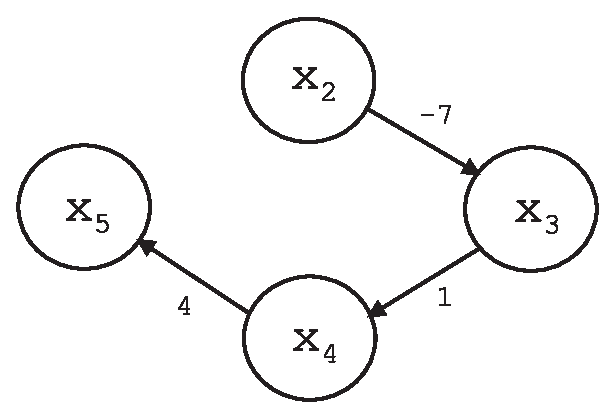
\includegraphics[height=2.0in]{s_iop0/impl01.eps}
\caption{System Of 3 Atomic Contraints}
\label{fig:siop0:sirn0:siac0:00}
\end{figure}

The three constraints in 
Figure \ref{fig:siop0:sirn0:siac0:00} imply a fourth
constraint ($x_5 - x_2 < -2$).  This fourth
implied constraint is shown with a dashed arrow in
Figure \ref{fig:siop0:sirn0:siac0:01}.  Note that
in Figures \ref{fig:siop0:sirn0:siac0:00} and
\ref{fig:siop0:sirn0:siac0:01}, the notion of implication
is viewed as ``shortest path closure'' of a graph (which is an equally
valid view).

\begin{figure}
\centering
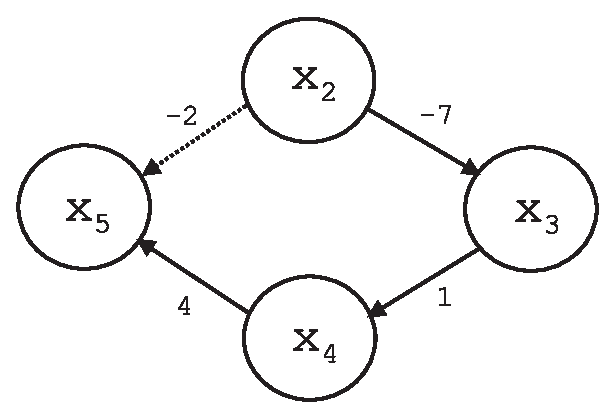
\includegraphics[height=2.0in]{s_iop0/impl02.eps}
\caption{System Of 3 Atomic Contraints With 4th Implied}
\label{fig:siop0:sirn0:siac0:01}
\end{figure}


%%%%%%%%%%%%%%%%%%%%%%%%%%%%%%%%%%%%%%%%%%%%%%%%%%%%%%%%%%%%%%%%%%%%%%%%%%%%%%%
%%%%%%%%%%%%%%%%%%%%%%%%%%%%%%%%%%%%%%%%%%%%%%%%%%%%%%%%%%%%%%%%%%%%%%%%%%%%%%%
%%%%%%%%%%%%%%%%%%%%%%%%%%%%%%%%%%%%%%%%%%%%%%%%%%%%%%%%%%%%%%%%%%%%%%%%%%%%%%%
\subsubsection{Contradiction Among Atomic Constraints}
%Subsubsection Tag: CAC0
\label{siop0:sirn0:scac0}

Contradictions among atomic constraints can also be stated in terms
of graph theory.  Specifically, any cycle 
in the graph with a negative sum of
edges represents a contradictory system of constraints,
and such a cycle is the only type of contradiction possible (although
we do not prove this second statement here).

At the level of the atomic constraint, the only contradictions
that may exist take the form of
(\ref{eq:siop0:sirn0:scac0:01})
through
(\ref{eq:siop0:sirn0:scac0:04}).

\begin{eqnarray}
\label{eq:siop0:sirn0:scac0:01} 
   & (x_i - x_j   <  d_{ij}) \wedge (x_i - x_j   >  \overline{d_{ij}}) \wedge (\overline{d_{ij}} \geq d_{ij}) & \\
\label{eq:siop0:sirn0:scac0:02}
   & (x_i - x_j   <  d_{ij}) \wedge (x_i - x_j \geq \overline{d_{ij}}) \wedge (\overline{d_{ij}}   >  d_{ij}) & \\
\label{eq:siop0:sirn0:scac0:03}
   & (x_i - x_j \leq d_{ij}) \wedge (x_i - x_j   >  \overline{d_{ij}}) \wedge (\overline{d_{ij}}   >  d_{ij}) & \\
\label{eq:siop0:sirn0:scac0:04}
   & (x_i - x_j \leq d_{ij}) \wedge (x_i - x_j \geq \overline{d_{ij}}) \wedge (\overline{d_{ij}}   >  d_{ij}) &
\end{eqnarray}

Contradictions in the form of
(\ref{eq:siop0:sirn0:scac0:01})
through
(\ref{eq:siop0:sirn0:scac0:04}) can be viewed as a cycle involving
only two variables (two nodes) in the graph.  As with implication, 
adjustments must be made for the distinction between
$\{ <, > \}$ and $\{ \leq , \geq \}$.

A negative-weight cycle in a graph can be viewed as a system of
constraints that (through implication, Section 
\ref{siop0:sirn0:siac0}), leads to a contradiction at the level
of the individual atomic constraint.  For example, consider
the following system of constraints, which leads to a graph with
a negative-weight cycle (Figure \ref{fig:siop0:sirn0:scac0:00}).

\begin{eqnarray}
\label{eq:siop0:sirn0:scac0:05} 
   x_5 - x_4 & < & 4 \\
\label{eq:siop0:sirn0:scac0:06}
   x_4 - x_3 & < & 1 \\
\label{eq:siop0:sirn0:scac0:07}
   x_3 - x_2 & < & -7 \\
\label{eq:siop0:sirn0:scac0:08}
   x_2 - x_5 & < & 1
\end{eqnarray}

\begin{figure}
\centering
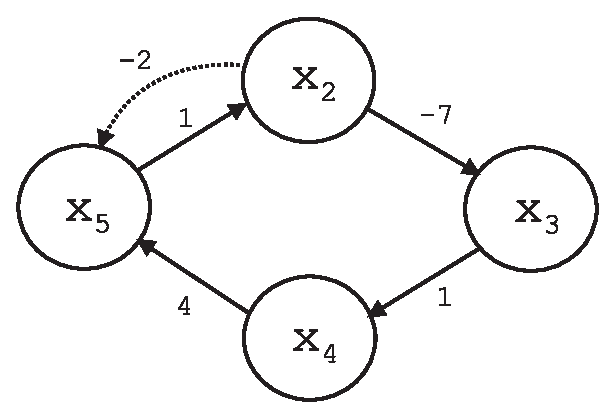
\includegraphics[height=2.0in]{s_iop0/cont01.eps}
\caption{Contradiction Among 4 Atomic Contraints}
\label{fig:siop0:sirn0:scac0:00}
\end{figure}

In Figure \ref{fig:siop0:sirn0:scac0:00},
note that 
(\ref{eq:siop0:sirn0:scac0:05}),
(\ref{eq:siop0:sirn0:scac0:06}),
and (\ref{eq:siop0:sirn0:scac0:07})
imply that $x_5 - x_2 < -2$ (shown with 
a dashed line in the figure), which contradicts
(\ref{eq:siop0:sirn0:scac0:08}).
It is straightforward to see that \emph{any} negative-weight
cycle in a graph of constraints will lead to a contradiction.

We should make formal how 
$\{ <, > \}$ versus $\{ \leq , \geq \}$ are to be treated for
detecting contradictions.  If \emph{all} constraints in the 
cycle involve $\leq$ rather than $<$, then a zero-weight cycle 
does not lead to a contradiction, and a strictly negative-weight
cycle is required to cause a contradiction.  On the other hand,
if at least one constraint in the cycle involves $<$, then both
zero-weight and negative-weight cycles lead to a contradiction.


%%%%%%%%%%%%%%%%%%%%%%%%%%%%%%%%%%%%%%%%%%%%%%%%%%%%%%%%%%%%%%%%%%%%%%%%%%%%%%%
%%%%%%%%%%%%%%%%%%%%%%%%%%%%%%%%%%%%%%%%%%%%%%%%%%%%%%%%%%%%%%%%%%%%%%%%%%%%%%%
%%%%%%%%%%%%%%%%%%%%%%%%%%%%%%%%%%%%%%%%%%%%%%%%%%%%%%%%%%%%%%%%%%%%%%%%%%%%%%%
\subsubsection{Canonical Form Of A Set Of Conjuncted Atomic Constraints}
%Subsection Tag: CFS0
\label{siop0:sirn0:scfs0}

The first question to address is how to assure a canonical
form of a set of atomic constraints (conjuncted together), each in the form
of (\ref{eq:siop0:sirn0:01}).  These results are well
established.  A very compact presentation of these ideas
is given in \cite[pp. 38-44]{bib:p:thsu2k:kglppet}.
Without a guaranteed unique canonical form, certain operations
become impossible; most notably comparison.


%%%%%%%%%%%%%%%%%%%%%%%%%%%%%%%%%%%%%%%%%%%%%%%%%%%%%%%%%%%%%%%%%%%%%%%%%%%%%%%
%%%%%%%%%%%%%%%%%%%%%%%%%%%%%%%%%%%%%%%%%%%%%%%%%%%%%%%%%%%%%%%%%%%%%%%%%%%%%%%
%%%%%%%%%%%%%%%%%%%%%%%%%%%%%%%%%%%%%%%%%%%%%%%%%%%%%%%%%%%%%%%%%%%%%%%%%%%%%%%
\paragraph{Reduction Of Constraints With Same Clocks But Different 
           Constants \mbox{\boldmath $d_{ij}$}:}

It is clear that if there are two [or more] constraints
naming the same variables in the same order with one constraint
tighter than the other, the ``looser'' constraint can be discarded.
For example, consider the two constraints in
(\ref{eq:siop0:sirn0:scfs0:01}) and (\ref{eq:siop0:sirn0:scfs0:02}).
It is clear that (\ref{eq:siop0:sirn0:scfs0:02}) may be discarded,
since (\ref{eq:siop0:sirn0:scfs0:01}) implies
(\ref{eq:siop0:sirn0:scfs0:02}).

\begin{eqnarray}
\label{eq:siop0:sirn0:scfs0:01} 
   x_2 - x_1 & \leq & 3 \\
\label{eq:siop0:sirn0:scfs0:02}
   x_2 - x_1 & \leq & 4
\end{eqnarray}

Similarly, given the two constraints 
(\ref{eq:siop0:sirn0:scfs0:03}) and 
(\ref{eq:siop0:sirn0:scfs0:04}), it is clear that
(\ref{eq:siop0:sirn0:scfs0:04}) can be discarded,
since (\ref{eq:siop0:sirn0:scfs0:03}) implies
(\ref{eq:siop0:sirn0:scfs0:04}).

\begin{eqnarray}
\label{eq:siop0:sirn0:scfs0:03} 
   x_2 - x_1 & < & 4 \\
\label{eq:siop0:sirn0:scfs0:04}
   x_2 - x_1 & \leq & 4
\end{eqnarray}


%%%%%%%%%%%%%%%%%%%%%%%%%%%%%%%%%%%%%%%%%%%%%%%%%%%%%%%%%%%%%%%%%%%%%%%%%%%%%%%
%%%%%%%%%%%%%%%%%%%%%%%%%%%%%%%%%%%%%%%%%%%%%%%%%%%%%%%%%%%%%%%%%%%%%%%%%%%%%%%
%%%%%%%%%%%%%%%%%%%%%%%%%%%%%%%%%%%%%%%%%%%%%%%%%%%%%%%%%%%%%%%%%%%%%%%%%%%%%%%
\paragraph{Reduction Of Contradictory Constraints Implying The Empty Set:}

Constraints can be specified which are contradictory.  Any subset
of contradictory constraints implies that the empty set is specified;
and that all constraints should be discarded and the 
\texttt{is\_empty} flag should be set (the canonical form of the 
empty set).

Section \ref{siop0:sirn0:scac0} has indicated that a necessary 
and sufficient
test for contradictory constraints is a negative-sum or non-positive-sum cycle 
(depending on whether the inequalities involve $\leq$ or $<$) in
the weighted directed graph corresponding to the set of constraints.


%%%%%%%%%%%%%%%%%%%%%%%%%%%%%%%%%%%%%%%%%%%%%%%%%%%%%%%%%%%%%%%%%%%%%%%%%%%%%%%
%%%%%%%%%%%%%%%%%%%%%%%%%%%%%%%%%%%%%%%%%%%%%%%%%%%%%%%%%%%%%%%%%%%%%%%%%%%%%%%
%%%%%%%%%%%%%%%%%%%%%%%%%%%%%%%%%%%%%%%%%%%%%%%%%%%%%%%%%%%%%%%%%%%%%%%%%%%%%%%
\paragraph{Atomic Constraints Involving Different Clocks:}

The final issue to consider in canonical forms is the nature of 
implications---under what circumstances can constraints be removed
because they are implied by other constraints?

In general (\cite[p. 288]{bib:b:modelchecking:clark1999}), 
the implications given in 
(\ref{eq:siop0:sirn0:siac0:01})
through 
(\ref{eq:siop0:sirn0:siac0:04})
hold.

Consider the system of constraints given by
(\ref{eq:siop0:sirn0:scfs0:25}) through 
(\ref{eq:siop0:sirn0:scfs0:27}).  Note that 
(\ref{eq:siop0:sirn0:scfs0:25}) $\wedge$ (\ref{eq:siop0:sirn0:scfs0:26})
$\Longrightarrow$ (\ref{eq:siop0:sirn0:scfs0:27}), so that 
(\ref{eq:siop0:sirn0:scfs0:27}) can be removed from the system
with no effect.

\begin{eqnarray}
\label{eq:siop0:sirn0:scfs0:25} 
   x_3 - x_2 & \leq & 7     \\
\label{eq:siop0:sirn0:scfs0:26}
   x_2 - x_1 & \leq & 3     \\
\label{eq:siop0:sirn0:scfs0:27}
   x_3 - x_1 & \leq & 10  
\end{eqnarray}

Note also that the implication chain resulting in the removal of 
constraints can be more indirect and involve more than three
constraints.  In 
(\ref{eq:siop0:sirn0:scfs0:28}) through 
(\ref{eq:siop0:sirn0:scfs0:31}) note that 
(\ref{eq:siop0:sirn0:scfs0:31}) can be discarded.

\begin{eqnarray}
\label{eq:siop0:sirn0:scfs0:28} 
   x_4 - x_3 & \leq & 7     \\
\label{eq:siop0:sirn0:scfs0:29}
   x_3 - x_2 & \leq & 3     \\
\label{eq:siop0:sirn0:scfs0:30}
   x_2 - x_1 & \leq & 3     \\
\label{eq:siop0:sirn0:scfs0:31}
   x_4 - x_1 & \leq & 14 
\end{eqnarray}

\cite{bib:b:modelchecking:clark1999} phrases 
this problem in terms of \index{shortest path closure}shortest 
path closure of a graph.
In general if there is a ``shorter'' directed path from variable to
variable than the one represented by a constraint, the constraint
is superfluous and
can be removed.  Thus, the implication problem can be
rephrased as a graph theory problem.

As before, some attention must be paid to the distinction between
$\{<, >\}$ and $\{ \leq, \geq \}$.  A constraint 
which represents an ``equal'' path may \index{corner-shaving@``corner-shaving''}
``shave a corner'' of
a region.  Consider the system given by 
(\ref{eq:siop0:sirn0:scfs0:32}) through
(\ref{eq:siop0:sirn0:scfs0:34}).  In this system,
(\ref{eq:siop0:sirn0:scfs0:34}) cannot be discarded without
including the point $(x_1=1, x_2=4)$ in the region,
which would change the region represented.

\begin{eqnarray}
\label{eq:siop0:sirn0:scfs0:32} 
   x_1       & \leq & 4     \\
\label{eq:siop0:sirn0:scfs0:33}
   x_2       & \geq & 1     \\
\label{eq:siop0:sirn0:scfs0:34}
   x_1 - x_2 & <    & 3 
\end{eqnarray}

Following the standard convention that
$x_0 \equiv 0$, (\ref{eq:siop0:sirn0:scfs0:32}) through
(\ref{eq:siop0:sirn0:scfs0:34}) can be rearranged into
the more standard form of (\ref{eq:siop0:sirn0:01}), 
and this more standard
form is given as
(\ref{eq:siop0:sirn0:scfs0:35}) through 
(\ref{eq:siop0:sirn0:scfs0:37}).  This standard form has the
weighted directed graph representation given by
Figure \ref{fig:siop0:sirn0:scfs0:02}.  A few paragraphs
earlier we made the statement that a constraint can be deleted
if a shorter or equivalent length path exists.  However, apparently
we must say in a case such as Figure \ref{fig:siop0:sirn0:scfs0:02} 
that the path $x_2 \rightarrow x_0 \rightarrow x_1$ is
``longer'' than the path $x_2 \rightarrow x_1$, and we must
treat $\{ \leq, \geq \}$ as ``longer'' 
than $\{<, >\}$ for purposes of deciding which constraints can
be removed.  It should also be clear that there are two categories
of path---those that consist exclusively of $\{ \leq, \geq \}$,
and those that do not.  Phrased differently, only one occurrence of
$\{<, >\}$ is required to create the shorter variety of path.

\begin{eqnarray}
\label{eq:siop0:sirn0:scfs0:35} 
   x_1 - x_0 & \leq & 4     \\
\label{eq:siop0:sirn0:scfs0:36}
   x_0 - x_2 & \leq & -1     \\
\label{eq:siop0:sirn0:scfs0:37}
   x_1 - x_2 & <    & 3 
\end{eqnarray}

\begin{figure}
\centering
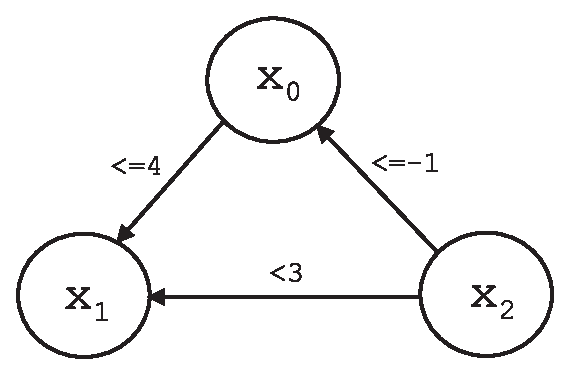
\includegraphics[height=2.0in]{s_iop0/leqeq01.eps}
\caption{``Corner-Shaving'' Of Region}
\label{fig:siop0:sirn0:scfs0:02}
\end{figure}

One question that comes to mind with ``corner-shaving'' is whether
in higher dimensional cases there may be more than one way to 
shave a corner.  It appears that there is not, but again, a proof
is beyond me (Dave Ashley) at this time.

%%%%%%%%%%%%%%%%%%%%%%%%%%%%%%%%%%%%%%%%%%%%%%%%%%%%%%%%%%%%%%%%%%%%%%%%%%%%%%%
%%%%%%%%%%%%%%%%%%%%%%%%%%%%%%%%%%%%%%%%%%%%%%%%%%%%%%%%%%%%%%%%%%%%%%%%%%%%%%%
%%%%%%%%%%%%%%%%%%%%%%%%%%%%%%%%%%%%%%%%%%%%%%%%%%%%%%%%%%%%%%%%%%%%%%%%%%%%%%%
\paragraph{Summary:}

It is believed that the following steps are adequate to ensure a canonical 
form of a conjunction of constraints of the form of
(\ref{eq:siop0:sirn0:01}):

\begin{enumerate}
\item If any cycle with a negative sum of weights appears in the constraints,
      the set is empty and the data structure should be marked to the
      canonical form for the empty set.
\item For constraints involving differences of the same clocks but with different 
      integer constant bounds, the looser constraints can always be removed.
\item Any constraints that do not represent the shortest path between variables
      can be removed.
\end{enumerate}

Again, I (Dave Ashley) am taking some of these approaches on faith for now.
A proof or two would help to reassure my fears.


%%%%%%%%%%%%%%%%%%%%%%%%%%%%%%%%%%%%%%%%%%%%%%%%%%%%%%%%%%%%%%%%%%%%%%%%%%%%%%%
%%%%%%%%%%%%%%%%%%%%%%%%%%%%%%%%%%%%%%%%%%%%%%%%%%%%%%%%%%%%%%%%%%%%%%%%%%%%%%%
%%%%%%%%%%%%%%%%%%%%%%%%%%%%%%%%%%%%%%%%%%%%%%%%%%%%%%%%%%%%%%%%%%%%%%%%%%%%%%%
\subsubsection{Inclusion}
%Subsection Tag: CFS0
\label{siop0:sirn0:sinc0}

To determine if a $A \subseteq B$ for two convex regions
$A$ and $B$, we can note that

\begin{equation}
\label{eq:siop0:sirn0:sinc0:00} 
(A \subseteq B) 
\Longleftrightarrow
(x \in A \rightarrow x \in B)
\Longleftrightarrow
(x \notin B \rightarrow x \notin A) .
\end{equation}

\noindent{}Thus, for every constraint in $B$, there must be
a constraint in $A$ (either directly stated or implied)
which is at least as strong.  This immediately suggests
an algorithm for determining if $A \subseteq B$, which is
provided as Figure \ref{fig:siop0:sirn0:sinc0:00}.

\begin{figure}
\begin{small}
\textbf{Input:} \\
\hspace*{0.15in}$A$ and $B$, two convex regions. \\
\textbf{Output:} \\
\hspace*{0.15in} \emph{TRUE} if $A \subseteq B$, \emph{FALSE} otherwise.\\
\textbf{begin} \\
\hspace*{0.15in}Determine if $A = \O$. \\
\hspace*{0.15in}Determine if $B = \O$. \\
\hspace*{0.15in}\textbf{if} $A = \O$ \textbf{then} return ``\emph{TRUE}''. \\
\hspace*{0.15in}\textbf{for} each constraint in $B$ \\
\hspace*{0.30in}\textbf{begin} \\
\hspace*{0.45in}\textbf{if} constraint involving same clocks exists in $A$ and is at least as tight \\
\hspace*{0.60in}\textbf{then} break (i.e. proceed to next iteration of loop)\\
\hspace*{0.45in}\textbf{elseif} shortest-path closure in $A$ can be found which is at least as tight \\
\hspace*{0.60in}\textbf{then} break \\
\hspace*{0.45in}\textbf{else} \\
\hspace*{0.60in}return ``\emph{FALSE}'' \\
\hspace*{0.30in}\textbf{end} \\
\hspace*{0.15in}return ``\emph{TRUE}'' \\
\textbf{end}
\end{small}
\caption{Algorithm For Determining Inclusion ($A \subseteq B$?)}
\label{fig:siop0:sirn0:sinc0:00}
\end{figure}

Note that it is not necessary for the constraints to
be in a strict canonical
form in order to apply the algorithm shown 
in Figure \ref{fig:siop0:sirn0:sinc0:00}.  However, it is necessary
to rule out $A, B = \O$.\footnote{Need to revisit this later---may not
actually be necessary.}


%%%%%%%%%%%%%%%%%%%%%%%%%%%%%%%%%%%%%%%%%%%%%%%%%%%%%%%%%%%%%%%%%%%%%%%%%%%%%%%
%%%%%%%%%%%%%%%%%%%%%%%%%%%%%%%%%%%%%%%%%%%%%%%%%%%%%%%%%%%%%%%%%%%%%%%%%%%%%%%
%%%%%%%%%%%%%%%%%%%%%%%%%%%%%%%%%%%%%%%%%%%%%%%%%%%%%%%%%%%%%%%%%%%%%%%%%%%%%%%
\subsubsection{Equality}
%Subsubsection Tag: EQU0
\label{siop0:sirn0:sequ0}

There are two possible algorithms for determining equality:

\begin{itemize}
\item A direct algorithm.
\item Defining equality with respect to inclusion, i.e.
      $(A \subseteq B) \wedge (B \subseteq A) \Longrightarrow (A = B)$.
\end{itemize}

For simplicity, we define equality in terms of inclusion (the second
approach above).


%%%%%%%%%%%%%%%%%%%%%%%%%%%%%%%%%%%%%%%%%%%%%%%%%%%%%%%%%%%%%%%%%%%%%%%%%%%%%%%
%%%%%%%%%%%%%%%%%%%%%%%%%%%%%%%%%%%%%%%%%%%%%%%%%%%%%%%%%%%%%%%%%%%%%%%%%%%%%%%
%%%%%%%%%%%%%%%%%%%%%%%%%%%%%%%%%%%%%%%%%%%%%%%%%%%%%%%%%%%%%%%%%%%%%%%%%%%%%%%
\subsection[Implementation Of Unions Of Convex Regions Of $\mathbb{R}^N$]
           {Implementation Of Unions Of Convex Regions Of \mbox{\boldmath $\mathbb{R}^N$}}
%Subsection Tag: URN0
\label{siop0:surn0}

Generally, if a CHM contains only a single path with no branches or loops,
the symbolic state in which the clocks may be at each location is a convex
region of $\mathbb{R}^N$.  This statement is true because the system starts 
at a known unique initial state (a point in $\mathbb{R}^N$, which is 
by definition convex), and each 
operation inherent in carrying the symbolic state through the single path
preserves the convexity.

However, when a CHM contains a cycle or multiple paths leading to a location,
the symbolic state can be a union of convex regions.  Such unions are 
treated as simple arrays of convex regions, and operations on such unions
are defined recursively in terms of the operations on convex regions.

The proposed form for representing a union of convex zones is an unordered array of
convex zones.  The difficulty in dealing with such unions is the difficulty of 
ensuring canonical forms.  This needs to be studied more deeply.


%%%%%%%%%%%%%%%%%%%%%%%%%%%%%%%%%%%%%%%%%%%%%%%%%%%%%%%%%%%%%%%%%%%%%%%%%%%%%%%
%%%%%%%%%%%%%%%%%%%%%%%%%%%%%%%%%%%%%%%%%%%%%%%%%%%%%%%%%%%%%%%%%%%%%%%%%%%%%%%
%%%%%%%%%%%%%%%%%%%%%%%%%%%%%%%%%%%%%%%%%%%%%%%%%%%%%%%%%%%%%%%%%%%%%%%%%%%%%%%
\subsubsection[Canonical Form Of A Union Of Convex Regions Of $\mathbb{R}^N$]
              {Canonical Form Of A Union Of Convex Regions Of \mbox{\boldmath $\mathbb{R}^N$}}
%Subsubsection Tag: CFU0
\label{siop0:surn0:cfu0}

Clearly, there are issues with canonical forms that need to be resolved
when unions are involved.

In particular, forming the union of multiple convex zones can lead to a number of outcomes,
and I'm not sure how to deal with all of those.  Here are the outcomes:

\begin{itemize}
\item The convex zones might not overlap at all.  In this case, 
      it would be guaranteed that taking the canonical form of
      each convex zone, combined with sorting the convex zones somehow,
      would lead to a canonical form.
\item One convex zone may be included in another.  There would be a straightforward
      test for this.  The included zone can be discarded.
\item One convex zone may overlap with another without a subset relationship.  
      In this case there are three outcomes.
      \begin{itemize}
      \item The two convex zones may have a union which forms a larger
            convex zone (for example, one can construct two rectangles
            which overlap in this way).  In this case the two zones can be
            combined.
      \item The two zones may overlap but their union may not be a 
            convex zone.  It may not be possible to adjust either zone
            without changing the region described.
      \item The two zones may overlap, and it may be possible to 
            adjust the zones without changing the region described.
            This immediately leads to concerns about uniqueness of 
            representation and canonical form.
      \end{itemize}
\end{itemize}

Note that some convex regions can be combined with other convex regions
to form another convex region.  For example, rectangles can be combined.

It is \emph{suspected} that the following procedure will result in a canonical
form:

\begin{itemize}
\item Arrange all convex regions in canonical form if necessary
      for subsequent algorithms.

\item Discard any empty sets.

\item Combine any two convex regions that result in any third
      convex region until no such regions can be combined
      any further.  This process would necessarily involve
      discarding inclusions.  (What is the algorithm for this?)

\item For any convex zones with overlap, adjust them downward
      in size as far as possible while not affecting the total
      region described.

\item Arrange convex regions in canonical form if necessary.

\item Sort the convex regions by some sort criteria.

\end{itemize}

Need some proofs to say that this is valid.  Need to think on this
further.


%%%%%%%%%%%%%%%%%%%%%%%%%%%%%%%%%%%%%%%%%%%%%%%%%%%%%%%%%%%%%%%%%%%%%%%%%%%%%%%
%%%%%%%%%%%%%%%%%%%%%%%%%%%%%%%%%%%%%%%%%%%%%%%%%%%%%%%%%%%%%%%%%%%%%%%%%%%%%%%
%%%%%%%%%%%%%%%%%%%%%%%%%%%%%%%%%%%%%%%%%%%%%%%%%%%%%%%%%%%%%%%%%%%%%%%%%%%%%%%
\subsection{Remarks On \swname{} Source Code}
%Subsection Tag: RHS0
\label{siop0:srhs0}


%%%%%%%%%%%%%%%%%%%%%%%%%%%%%%%%%%%%%%%%%%%%%%%%%%%%%%%%%%%%%%%%%%%%%%%%%%%%%%%
%%%%%%%%%%%%%%%%%%%%%%%%%%%%%%%%%%%%%%%%%%%%%%%%%%%%%%%%%%%%%%%%%%%%%%%%%%%%%%%
%%%%%%%%%%%%%%%%%%%%%%%%%%%%%%%%%%%%%%%%%%%%%%%%%%%%%%%%%%%%%%%%%%%%%%%%%%%%%%%
\subsubsection{Source And Documentation File Manifest}
%Subsubsection Tag: SDF0
\label{siop0:srhs0:ssdf0}

This section contains a description of every file of
\swname{} and its documentation.  All of the files listed
below are maintained under version control (\index{CVS}CVS).

\begin{enumerate}
\item \index{mf\_lex.c@\texttt{mf\_lex.c}}%
      \texttt{c:$\backslash$swprojsb$\backslash$hyreach$\backslash$mf\_lex.c} \\
      (File mnemonic:  \emph{m}odel \emph{f}ile \emph{lex}ical analysis.)  Contains functions
      which scan the model input file, lexically analyze it, and deliver a 
      complete ordered list of tokens (in dynamic
      memory) representing the contents of the model input file.
\item \index{mf\_lex.h@\texttt{mf\_lex.h}}%
      \texttt{c:$\backslash$swprojsb$\backslash$hyreach$\backslash$mf\_lex.h} \\
      Header file for \texttt{mf\_lex.c}.
\end{enumerate}


%%%%%%%%%%%%%%%%%%%%%%%%%%%%%%%%%%%%%%%%%%%%%%%%%%%%%%%%%%%%%%%%%%%%%%%%%%
\noindent\begin{figure}[!b]
\noindent\rule[-0.25in]{\textwidth}{1pt}
\begin{tiny}
\begin{verbatim}
$RCSfile: s_iop0.tex,v $
$Source: /cvsroot/esrg/sfesrg/esrgpcpj/hyreach/doc/hyreachm/s_iop0/s_iop0.tex,v $
$Revision: 1.11 $
$Author: dtashley $
$Date: 2002/01/29 17:04:00 $
\end{verbatim}
\end{tiny}
\noindent\rule[0.25in]{\textwidth}{1pt}
\end{figure}
%%%%%%%%%%%%%%%%%%%%%%%%%%%%%%%%%%%%%%%%%%%%%%%%%%%%%%%%%%%%%%%%%%%%%%%%%%
%$Log: s_iop0.tex,v $
%Revision 1.11  2002/01/29 17:04:00  dtashley
%Version control info added, and minor edits.
%
%Revision 1.10  2001/12/01 21:29:54  dtashley
%Safety checkin after edits.
%
%Revision 1.9  2001/11/29 20:15:16  dtashley
%Safety checkin after edits.
%
%Revision 1.8  2001/11/28 19:48:58  dtashley
%Edits.
%
%Revision 1.7  2001/11/09 19:38:16  dtashley
%Safety checkin.
%
%Revision 1.6  2001/11/07 19:52:53  dtashley
%Edits.
%
%Revision 1.5  2001/11/01 06:49:08  dtashley
%Nightly safety check in.
%
%Revision 1.4  2001/10/31 04:31:37  dtashley
%Nightly safety checkin.
%
%Revision 1.3  2001/10/25 05:32:40  dtashley
%Evening safety checkin after edits.
%
%Revision 1.2  2001/09/26 04:51:13  dtashley
%Edits.
%
%Revision 1.1  2001/09/26 02:31:14  dtashley
%Initial checkin, and some edits of main TEX file.
%
%End of S_IOP0.TEX.
